\documentclass[10pt]{article}
\usepackage[margin=1.35in]{geometry}
\usepackage[utf8]{inputenc}
\usepackage[T1]{fontenc}
\usepackage{amsmath,amssymb,amsfonts}
\usepackage{booktabs}
\usepackage{graphicx}
\usepackage{hyperref}
\usepackage{url}
\usepackage{natbib}
\usepackage[capitalize]{cleveref}

\title{Shortcut-Masked Calibration for Synthetic SMS Filtering}

\author{Anonymous Authors\\
Paper under double-blind review}

\begin{document}
\maketitle

\begin{abstract}
Compact classifiers can overfit to surface tokens rather than underlying semantics. We study Shortcut-Masked Calibration (SMC), pairing token masking with post-hoc temperature scaling. On our synthetic benchmark, SMC achieves 91.4\% Macro-F1 and 0.032 Expected Calibration Error (ECE).
\end{abstract}

\section{Introduction}
\label{sec:intro}
Neural classifiers frequently exploit unintended decision rules under distribution shift \citep{Geirhos2020ShortcutLearning}. Furthermore, post-hoc calibration is critical for reliable confidence estimates \citep{Guo2017CalibrationModern}.

\section{Related Work}
\label{sec:related_work}
\subsection{Model Calibration}
Post-hoc temperature scaling provides an effective calibration mechanism on held-out validation logits \citep{Guo2017CalibrationModern}.

\subsection{Shortcut Mitigation}
Deep models often rely on spurious surface cues \citep{Geirhos2020ShortcutLearning}; masking surface tokens targets this failure mode.

\section{Methodology}
\label{sec:method}
\subsection{Surface Token Masking}
We mask URL and phone surface tokens prior to encoding, following the formulation in our research notes.

\subsection{Post-Hoc Temperature Scaling}
Given logits $z(x)$, calibrated probabilities are computed as
\begin{equation}
  p(y \mid x) = \text{softmax}(z(x) / \tau), \quad \tau > 0.
\end{equation}

\section{Experiments}
\label{sec:experiments}
\subsection{Experimental Setup}
All runs use a 5-fold group split with fixed seed 42 and batch size 32, evaluating Macro-F1 (\%) and ECE.

\subsection{Main Results}
\cref{tab:main} and \cref{fig:accuracy} summarize quantitative results from the experimental log.

\begin{table}[t]
\centering
\caption{Main quantitative results on the synthetic benchmark (5-fold group split, seed 42).}
\label{tab:main}
\begin{tabular}{lcc}
\toprule
Method & Macro-F1 (\%) $\uparrow$ & ECE $\downarrow$ \\
\midrule
TF-IDF + LR & 84.2 & 0.091 \\
Compact Encoder (Unmasked) & 88.5 & 0.064 \\
Compact Encoder + SMC (Ours) & \textbf{91.4} & \textbf{0.032} \\
\bottomrule
\end{tabular}
\end{table}

\begin{figure}[t]
\centering
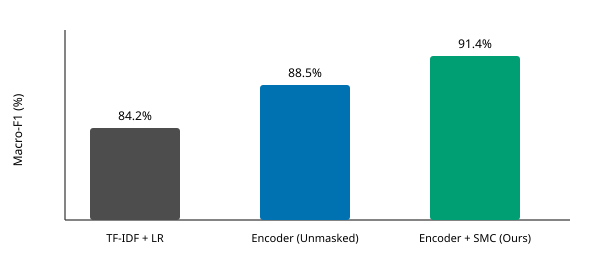
\includegraphics[width=0.95\linewidth]{figures/fig_accuracy_bar.svg}
\caption{Macro-F1 comparison across TF-IDF + LR, Unmasked Encoder, and SMC on the synthetic sample benchmark.}
\label{fig:accuracy}
\end{figure}

\section{Limitations}
\label{sec:limitations}
This validation study is evaluated solely on synthetic sample records; real-world multilingual deployment requires full corpus evaluation.

\section{Conclusion}
\label{sec:conclusion}
Combining surface-token masking with temperature scaling improves both Macro-F1 (91.4\%) and ECE (0.032) on the synthetic benchmark.

\section*{Reproducibility Statement}
All experiments use seed 42, batch size 32, and a 5-fold group split as recorded in the experimental log.

\bibliographystyle{plainnat}
\bibliography{references}

\end{document}
